\documentclass[debug,a0paper,portrait]{xebaposter}

\usepackage{url}
\usepackage{amsmath}
\usepackage{amssymb}
%\usepackage{relsize}
%\usepackage{graphicx}
\usepackage{multicol}
\usepackage{xecolor}
%\usepackage[verbose]{wrapfig}
\graphicspath{{images/}}
\usepackage[inline]{enumitem}% for making inline list.
\setlist{noitemsep}% Save space in lists.

\usepackage{xepersian}
\settextfont{Yas}

 %%%%%%%%%%%%%%%%%%%%%%%%%%%%%%%%%%%%%%%%%%%%%%%%%%%%%%%%%%%%%%%%%%%%%%%%%%%%%%%%
 %%%% Some math symbols used in the text
 %%%%%%%%%%%%%%%%%%%%%%%%%%%%%%%%%%%%%%%%%%%%%%%%%%%%%%%%%%%%%%%%%%%%%%%%%%%%%%%%
 % Format 
% \newcommand{\RotUP}[1]{\begin{sideways}#1\end{sideways}}


 %%%%%%%%%%%%%%%%%%%%%%%%%%%%%%%%%%%%%%%%%%%%%%%%%%%%%%%%%%%%%%%%%%%%%%%%%%%%%%%%
 % Multicol Settings
 %%%%%%%%%%%%%%%%%%%%%%%%%%%%%%%%%%%%%%%%%%%%%%%%%%%%%%%%%%%%%%%%%%%%%%%%%%%%%%%%
% \setlength{\columnsep}{0.7em}
% \setlength{\columnseprule}{0mm}


%% Begin of Document
%%%%%%%%%%%%%%%%%%%%%%%%%%%%%%%%%%%%%%%%%%%%%%%%%%%%%%%%%%%%%%%%%%%%%%%%%%%%%
\begin{document}
%%% Setting User Defined Background %%%%%%%%%%%%%%%%%%%%%%%%%%%%%%%%%%%%%%%%%%%%%%
%if you want to use your preferred background, you should set background=user in poster settings.
\background{
  \begin{bidi@tikzpicture}[remember picture,overlay,opacity=.3]%
    \fill [green!20!yellow] {(current page.south east) rectangle (current page.north west)};%
	\draw (current page.north west)+(-2em,2em) node[anchor=north west,opacity=.3]
	{
\includegraphics[width=1.1\textwidth]{logo}};
  \end{bidi@tikzpicture}%
} 
%%%%%%%%%%%%%%%%%%%%%%%%%%%%%%%%%%%%%%%%%%%%%%%%%%%%%%%%%%%%%%%%%%%%%%%%%%%%%
%% Here starts the poster
%%---------------------------------------------------------------------------
%% Format it to your taste with the options
%%%%%%%%%%%%%%%%%%%%%%%%%%%%%%%%%%%%%%%%%%%%%%%%%%%%%%%%%%%%%%%%%%%%%%%%%%%%%
      \definecolor{silver}{cmyk}{0,0,0,0.3}
      \definecolor{yellow}{cmyk}{0,0,0.9,0.0}
      \definecolor{reddishyellow}{cmyk}{0,0.22,1.0,0.0}
      \definecolor{black}{cmyk}{0,0,0.0,1.0}
      \definecolor{darkYellow}{cmyk}{0,0,1.0,0.5}
      \definecolor{darkSilver}{cmyk}{0,0,0,0.1}

      \definecolor{lightyellow}{cmyk}{0,0,0.3,0.0}
      \definecolor{lighteryellow}{cmyk}{0,0,0.1,0.0}
      \definecolor{lighteryellow}{cmyk}{0,0,0.1,0.0}
      \definecolor{lightestyellow}{cmyk}{0,0,0.05,0.0}

      \begin{poster}%
      % Poster Options
      {
      eyecatcher=true,
      % Color style
      bgColorOne=green!40!yellow!30,%lighteryellow,
      bgColorTwo=yellow,
      borderColor=reddishyellow,
      headerColorOne=yellow,
      headerColorTwo=reddishyellow,
      headerFontColor=cyan,
      boxColorOne=lightyellow,      
      boxColorTwo=lighteryellow,
      % Format of textbox
      textborder=rounded,
      % Format of text header
      headerborder=closed,
      headerheight=.087\textheight,
      headershape=roundedleft,
      headershade=plain,
%      headerfont=\Large, %Sans Serif
      boxshade=plain,
      background=plain,% user,
      linewidth=2pt,
      grid=false, % show a grid mesh on poster, it's useful for debugging.
      }
 % Eye Catcher
 {
      
\includegraphics[height=0.07\textheight]{logo}
 }
 % Title
 {طراحی پوستری زیبا و در خور با کمک کلاس \lr{xebaposter} (راهنمـــــــــــــــا)
}
 % Authors
 {\large \lr{Brian Amberg}, \lr{Reinhold Kainhofer}, سیّدمحمّدجواد رضویان
 \\%[1em]
 {\normalsize\texttt{\lr{javadr@parsilatex.com, reinhold@kainhofer.com, baposter@brian-amberg.de}}}}
 % University logo
 {
\begin{tabular}{r}
    
\includegraphics[height=0.07 \textheight]{logo}\\
\end{tabular}
 }
% \end{poster}
% \end{document}
%%%%%%%%%%%%%%%%%%%%%%%%%%%%%%%%%%%%%%%%%%%%%%%%%%%%%%%%%%%%%%%%%%%%%%%%%%%%%%
%%% Now define the boxes that make up the poster
%%%---------------------------------------------------------------------------
%%% Each box has a name and can be placed absolutely or relatively.
%%% The only inconvenience is that you can only specify a relative position 
%%% towards an already declared box. So if you have a box attached to the 
%%% bottom, one to the top and a third one which should be inbetween, you 
%%% have to specify the top and bottom boxes before you specify the middle 
%%% box.
%%%%%%%%%%%%%%%%%%%%%%%%%%%%%%%%%%%%%%%%%%%%%%%%%%%%%%%%%%%%%%%%%%%%%%%%%%%%%%

 %%%%%%%%%%%%%%%%%%%%%%%%%%%%%%%%%%%%%%%%%%%%%%%%%%%%%%%%%%%%%%%%%%%%%%%%%%%%%%
\begin{posterbox}[name=introduction,column=0,row=0,headershape=smallrounded]%
{\textxecolor{red}{مقدمه}}
 %%%%%%%%%%%%%%%%%%%%%%%%%%%%%%%%%%%%%%%%%%%%%%%%%%%%%%%%%%%%%%%%%%%%%%%%%%%%%%
همانطوری که می‌دانید یکی از نیازهای جامعه علمی طراحی پوستر است زیرا که در برخی کنفرانس‌ها نویسنده مقاله تنها مجاز به ارائه پوستر 
می‌گردد. در این راستا یک بسته بسیار ساده به نام \texttt{a0poster} وجود دارد که در عین سادگی کار با آن، قابلیت‌های زیادی ندارد.
از طرفی دیگر بسته‌های زیبایی برای تولید پوستر توسط افرادی دیگر طراحی شده است 
از جمله \texttt{baposter}\footnote{\url{http://www.brian-amberg.de/uni/poster/}}
 و \texttt{beamerposter}. 
متاسفانه این بسته‌ها با متون راست به چپ، خصوصاً فارسی کار نمی‌کنند. از آنجایی که بسته \texttt{baposter} 
بر پایه \texttt{tikz} طراحی شده است و جناب آقای دکتر وفا خیلقی خالق 
بسته‌های \texttt{bidi} و \texttt{xepersian} امکان پشتیبانی از متون 
راست به چپ را در تصاویر تولیدی بسته \texttt{tikz} فراهم آورده‌اند پس بدین سبب به سراغ این بسته رفته و با تغییراتی در آن، 
این بسته را با متون راست به چپ خصوصا فارسی سازگار نموده و نام \texttt{xebaposter} را بر آن برگزیدیم%
\footnote{نگارنده ابتدا نام \lr{baposterRL} را انتخاب کرده بود لکن با پیشنهاد دکتر محمود امین‌طوسی نام فعلی را برگزید.}
--بخوانید زیباپوستر--. 
البته ناگفته نماند که پوسترهای تولیدی با بسته \texttt{beamerposter} زیبایی زاید الوصوفی دارند لکن به سبب اینکه بسته‌های 
بایدی و زی‌پرشین فعلا از بسته \texttt{beamer} پشتیبانی نمی‌کنند --آنهم به سبب وجود باگ‌هایی در موتور زی‌تک-- امکان 
فارسی‌سازی این بسته وجود نداشت پس بدین سبب تنها انتخابمان همان بسته اولیه \texttt{baposter} شد.
متاسفانه به سبب وجود باگ‌\footnote{گزارش شده در \url{http://qa.parsilatex.com/10715} 
و \url{http://tex.stackexchange.com/questions/262877}} در موتور زی‌لتک فعلاً ویژگی محوشدگی رنگ را نخواهیم داشت.%
\footnote{برای مشاهده
نمونه‌هایی از این بسته‌ها می‌توانید به \url{http://www.latextemplates.com/cat/conference-posters} مراجعه نمایید.}
\end{posterbox}
 %%%%%%%%%%%%%%%%%%%%%%%%%%%%%%%%%%%%%%%%%%%%%%%%%%%%%%%%%%%%%%%%%%%%%%%%%%%%%%
\begin{posterbox}[name=usage,column=1,span=1,headershape=rounded,textborder=rectangle
,textborder=faded]{نحوه کاربرد}
محیط اصلی پوستر، محیط \texttt{poster} است با ساختاری مانند ذیل:
\begin{latin}
\vspace{-2mm}
\begin{verbatim}
\begin{poster}
    { key=value options }
    { Eye Catcher, empty 
       if option eyecatcher=no}
    { Poster Title }
    { Poster Authors }
    { University Logo}
    
    Definition of the boxes
\end{poster}
\end{verbatim}
\end{latin}
\end{posterbox}
 %%%%%%%%%%%%%%%%%%%%%%%%%%%%%%%%%%%%%%%%%%%%%%%%%%%%%%%%%%%%%%%%%%%%%%%%%%%%%%
\begin{posterbox}[name=classoption,column=2,span=1,headershape=rectangle,textborder=roundedsmall]
{گزینه‌های کلاس}
 %%%%%%%%%%%%%%%%%%%%%%%%%%%%%%%%%%%%%%%%%%%%%%%%%%%%%%%%%%%%%%%%%%%%%%%%%%%%%%
\begin{itemize}
    \item \texttt{portrait/landscape}: طرح‌بندی صفحه
    \item \texttt{a0paper, a1paper, a2paper, a3paper, a4paper, archE}: سایز صفحات از پیش تعریف‌شده
    \item \texttt{paperwidth=length, paperheight=length}: تنظیم عرض/ارتفاع صفحه. 
    این گزینه‌ها را بهیچوجه با صفحات از پیش‌تعریف شده بکار نبرید.
    \item \texttt{margin=length}: حاشیه صفحه
    \item \lr{\texttt{fontscale=real number}}:
    \item \texttt{showframe}: نمایش فریم. این گزینه‌ در اشکال‌زدایی بکار می‌آید.
\end{itemize}
\end{posterbox}

 %%%%%%%%%%%%%%%%%%%%%%%%%%%%%%%%%%%%%%%%%%%%%%%%%%%%%%%%%%%%%%%%%%%%%%%%%%%%%%
\begin{posterbox}[name=posteroption,column=1,span=2,below=classoption]{گزینه‌های محیط \lr{poster}}
 %%%%%%%%%%%%%%%%%%%%%%%%%%%%%%%%%%%%%%%%%%%%%%%%%%%%%%%%%%%%%%%%%%%%%%%%%%%%%%
%\begin{multicols}{2}
\begin{itemize}
    \item \texttt{grid={yes,no}}: .نمایش یک گرید. این گزینه در فاز طرح‌بندی پوستر بکار آید.
    \item \texttt{columns=4}:  تعداد ستون‌ها. 
     (در حالت افقی ۴ و در حالت عمودی مقدار پیش‌فرض ۳ است و حداکثر تعداد ستون‌ها ۶ است.)
    \item \texttt{colspacing=length}: فاصله بین‌ستون‌های پوستر.
    \item \texttt{headerheight=length}: ارتفاع بخش سرآمد پوستر. مقدار پیش‌فرض آن {\verb|0.1\textheight|} است.
    \item \lr{\texttt{background=poster background type}}: پشت‌زمینه پوستر را تعیین می‌کند که می‌تواند مقادیر زیر را بگیرد:
    \begin{enumerate}
        \item \texttt{plain}: رنگ پشت‌زمینه را رنگ \texttt{bgColorOne} می‌گذارد.
        \item \texttt{user}: با دستور \verb|\background{...}| پشت‌زمینه مطلوبتان را می‌توانید طراحی نمایید.
        \item \texttt{none}: بدون پشت زمینه.
    \end{enumerate}
    \item \lr{\texttt{bgColorOne=pgf color name}}: رنگ اول پشت‌زمینه. در حالت \texttt{plain} تنها همین رنگ بکار می‌رود.
    \item \lr{\texttt{bgColorTwo=pgf color name}}: رنگ دوم پشت‌زمینه.
    \item \lr{\texttt{eyecatcher={yes,no}}}: تعیین می‌کند که آیا آی‌کچر در سرآمد پوستر به نمایش درآید یا نه. 
    این تصویر در سمت راست عنوان قرار خواهد گرفت.
\end{itemize}
%\end{multicols}
\end{posterbox}
%%%%%%%%%%%%%%%%%%%%%%%%%%%%%%%%%%%%%%%%%%%%%%%%%%%%%%%%%%%%%%%%%%%%%%%%%%%%%%
\begin{posterbox}[name=posterboxoption,column=1,span=2,below=posteroption,textborder=none
,headershape=rectangle,headerborder=none,textborder=coils]
{گزینه‌های محیط \lr{posterbox}}
    هر جعبه پوستر باید در یک محیط \texttt{posterbox} به صورت زیر تعریف گردد:
\begin{latin}
\vspace{-3mm}
\begin{verbatim}
    \begin{posterbox}[ key=value options ]{ PosterBox Title }
        Contents
    \end{posterbox}
\end{verbatim}
\end{latin}
\begin{itemize}
    \item \lr{\texttt{name=box name}}: نام جعبه را مشخص می‌کند. این نام در تعیین موقعیت دیگر جعبه‌ها نسبت به آن بکار آید.
    \item \lr{\texttt{column=column number}}: مشخص می‌کند که جعبه در کدام ستون قرار گیرد 
    --شماره ستون‌ها از صفر شروع می‌شود--.
    \item \lr{\texttt{span=column span}}:    
    مشخص می‌کند که جعبه شامل چند ستون از پوستر خواهد بود --مقدار پیش‌فرض عدد یک است--. 
    \item \lr{\texttt{borderColor=pgf color name}}:
    رنگ مورد استفاده در حاشیه جعبه‌ها. 
    \item \lr{\texttt{headerColorOne=pgf color}}:
    رنگ اول عنوان جعبه.
    \item \lr{\texttt{headerColorTwo=pgf color name}}:
    رنگ دوم عنوان جعبه.
    \item \lr{\texttt{textborder=border type}}:
    نوع حاشیه پایین جعبه را تعیین می‌کند که خود شامل انواع زیر است:
    
    \centerline{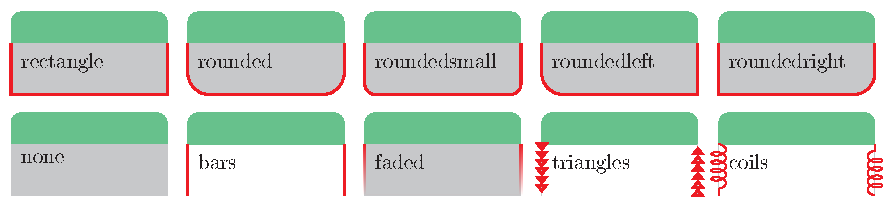
\includegraphics[scale=0.7]{docs-boxshape}}
    \item \lr{\texttt{headerborder=header border type}}:
    آن بخشی از جعبه که پیرامون عنوان قرار می گیرد را تعیین می‌کند:
    
    \centerline{
\includegraphics[scale=0.7]{docs-headerborder}}
    \item \lr{\texttt{headershape=header border shape}}:
    نوع آرایش عنوان جعبه را مشخص می‌کند:
    
    \centerline{
\includegraphics[scale=0.7]{docs-headershape}}
    \item \lr{\texttt{headershade=type of header shading}}:
    
        \begin{enumerate*}[label=\arabic*)]
            \item\texttt{plain} 
            \item\texttt{shade-lr} 
            \item\texttt{shade-rl} 
            \item\texttt{shade-tb}
            \item\texttt{shade-tb-inverse}
        \end{enumerate*}
        
    \item \lr{\texttt{boxshade}}:
    
        \begin{enumerate*}[label=\arabic*)]
            \item\texttt{plain} 
            \item\texttt{shade-lr} 
            \item\texttt{shade-tb}
            \item\texttt{plain} 
            \item\texttt{none}
        \end{enumerate*}
    \item \lr{\texttt{headerfont=font definition}}:
    دستوری که قبل از حروفچینی عنوان جعبه قرار داده می‌شود.
    \item \lr{\texttt{headerFontColor=pgf color name}}:
    رنگ قلم عنوان جعبه.
    \item \lr{\texttt{linewidth=length}}:
    عرض خطوط مورد استفاده در ترسیم پوستر
    \item \lr{\texttt{above=box name,below=box name,aligned=box name,bottomaligned=box name}}: 
    نام جعبه‌ای را مشخص می‌کند که این جعبه باید نسبت به آن ترازبندی شود.
\end{itemize}
\vspace{-2mm}
    نکته‌ای که باید در چینش جعبه‌ها در نظر داشته باشید این است که مکان جعبه‌ها می‌توانند به صورت نسبی یا دقیق تعیین شود. 
    اگر برای مثال جعبه ب قرار است دقیقاً بین جعبه‌های الف و ج قرار گیرد 
    آنگاه این دو جعبه اخیر حتماً باید پیش از جعبه ب تعریف شوند، در غیر اینصورت سبب تولید خطا می‌گردد. ضمنا می‌توانید بدون 
    تعیین این پارامترها چینش جعبه‌ها را به صورت خودکار و بهمان ترتیب تعریف به خود بسته واگذار نمایید.
\end{posterbox}
%%%%%%%%%%%%%%%%%%%%%%%%%%%%%%%%%%%%%%%%%%%%%%%%%%%%%%%%%%%%%%%%%%%%%%%%%%%%%%
\begin{posterbox}[name=imagedataset,column=0,span=1,below=introduction,textborder=roundedleft]
{\textxecolor{blue}{اجزاء تشکیل دهنده زیباپوستر}}
 %%%%%%%%%%%%%%%%%%%%%%%%%%%%%%%%%%%%%%%%%%%%%%%%%%%%%%%%%%%%%%%%%%%%%%%%%%%%%%
زیباپوستر صفحه پوستر را به دو بخش سرآمد  و محتوی تقسیم می‌کند. خود سرآمد نیز از سه بخش آی‌کچر، عنوان و لوگوی موسسه تشکیل 
شده است که بهمین ترتیب نمایش داده می‌شود. بخش آی‌کچر اختیاری است و می‌توان با گزینه \texttt{eyecatcher} آن را فعال یا غیرفعال 
نمود(\texttt{true,false}). در صورت عدم وجود آی‌کچر، عنوان و نام نویسنده‌(ها) راست چین خواهد شد و در صورت وجود آن به صورت 
وسط‌چین در خواهند آمد.

بخش محتوای پوستر شامل تعدادی جعبه \texttt{tikz} است که حاوی مطالب پوستر خواهند بود. این جعبه‌ها از طریق 
محیط \texttt{posterbox} تعریف می‌شوند. تمامی این جعبه‌ها باید درون محیط \lr{poster} تعریف شده باشند. 
هر جعبه نیز از دو بخش عنوان و محتوی تشکیل شده است. و نهایتا پشت زمینه پوستر است که در حال حاضر تنها می‌تواند یک رنگ ساده 
باشد و یا اصلا چیزی نباشد و یا به اختیار کاربر قرار گیرد تا برای مثال در صورت تمایل یک تصویر پشت زمینه قرار دهد --البته همانطور که 
در بالا اشاره گردید برخی قابلیت‌های محیط \lr{tikz} از جمله محوشدگی قابل استفاده نمی‌باشند--. 
\end{posterbox}
 %%%%%%%%%%%%%%%%%%%%%%%%%%%%%%%%%%%%%%%%%%%%%%%%%%%%%%%%%%%%%%%%%%%%%%%%%%%%%%
\begin{posterbox}[name=setting,column=0,span=1,below=imagedataset%
,headerFontColor=brown,textborder=roundedright,headershape=roundedright]
{\textxecolor{brown}{تنظیمـــــــــات (عمومی یا محلی؟!)}}
 %%%%%%%%%%%%%%%%%%%%%%%%%%%%%%%%%%%%%%%%%%%%%%%%%%%%%%%%%%%%%%%%%%%%%%%%%%%%%%
کاربر می‌توانید تنظیماتی را که برای رنگ و حالت جعبه‌ها تعریف شده است را به کلی یا جزئی تغییر دهد. بدین معنی که برای یکبار همان
ابتدای تعریف محیط \lr{poster} که این تنظیمات تعریف می‌شوند بر تمامی جعبه‌ها قابل اعمال هستند لکن این امکان نیز وجود دارد 
که هر جعبه را به طور خاص شخصی‌سازی نمود. در این پوستر سعی شده تا با اتخاذ 
شخصی‌سازی هر جعبه گزینه‌های مختلف موجود تا آنجا که ممکن است نشان داده شود. 
\end{posterbox}
 %%%%%%%%%%%%%%%%%%%%%%%%%%%%%%%%%%%%%%%%%%%%%%%%%%%%%%%%%%%%%%%%%%%%%%%%%%%%%%
\begin{posterbox}[name=ack,column=0,span=1,below=setting,textborder=faded,
,textborder=triangles]{قدردانی}
 %%%%%%%%%%%%%%%%%%%%%%%%%%%%%%%%%%%%%%%%%%%%%%%%%%%%%%%%%%%%%%%%%%%%%%%%%%%%%%
با تشکر از دکتر \lr{Brian} خالق کلاس پوستر و تشکر ویژه از جناب آقای دکتر وفا خیلقی بخاطر زحماتی که برای فارسی‌نویسی در
محیط زی‌لاتک انجام‌ داده‌اند و دکتر محمود امین‌طوسی به سبب پیشنهاد نام زیباپوستر و گروه پارسی‌لاتک برای تست این کلاس.
\end{posterbox}
 %%%%%%%%%%%%%%%%%%%%%%%%%%%%%%%%%%%%%%%%%%%%%%%%%%%%%%%%%%%%%%%%%%%%%%%%%%%%%%
\end{poster}
\end{document}
